\chapter{Anticipated contribution} \label{contribution}
The main contribution of my research to the software engineering and software process community is the development and evaluation of a previously unexplored approach to discovering of recurrent behaviors in software process through the data mining of low-level process and product artifacts.

The knowldege developed through the experimental work, and evaluation of the approach taken, will be another contribution of my research. By performing these experiments, I also hoping to discover new patterns in the software process thereby improving our knowledge about it.

The software framework and data mining toolkit which I will develop for my research will be integrated with the existing family of Hackystat tools and made available as open source, thus contributing to the software-engineering community.

\section{Estimated Timeline}
By the beginning of the Fall'09 semester, I plan to design a taxonomy and implement a low-level software process artifact abstractions into a symbolic representation for the classroom experiments. The current database schema will be extended for storing these data and indexes. Immediately after that, I will proceed with the implementation of fundamental algorithms for sequential patterns mining from the time-points and time-interval data. My goal is to have a first-generation data model and KDD toolkit to be available for use before in-class development starts. 

Based on the Fall'09 classroom experiment experience, I will extend and fine-tune my system for the Spring'10 software engineering class, during which I plan to evaluate a final version of my system. The results of these two classroom experiments, the description of designed methods and developed software will constitute a peer-reviewed publication which I plan finish by Summer'10.

The MSR Challenge 2010 is announced to happen early May'10. I plan to design SCM data mining toolkit and perform pilot experiments by early January'10 submitting an abstract. If accepted, I will prepare and submit a research paper following the Challenge timeline.

I plan to be working on my thesis during Fall'09, Spring'10 and Summer'10 semesters. During the Fall'10 semester I plan to finish my work and defend the dissertation.

\begin{figure}[tbp]
   \centering
   \includegraphics[height=73mm]{timeline.eps}
   \caption{Proposed Trajectory development timeline.}
   \label{fig:timeline}
\end{figure}